
% WARN: partito da pagina 26 del pdf 1
% TODO: arrivato a pagina 52


\subsection{IT come commodity}
LE tecnologie infrastrutturali subiscono rapide crescite causa investimenti giganteschi
che causano un calo dei prezzi.

\subsection{Infrastrutture}
Le infrastrutture sono spinte principalmente da investimenti privati e governative,
la rete a banda larga è un'infrastruttura centrale per la competitività delle aziende e 
di un paese.

Ad oggi l'Italia investe per ottenere una velocità di banda non inferiore a 1 Gbit/s su
tutto il territorio italiano entro il 2026(limite europeo 2030).



\subsection{Evoluzione dei sistemi informativi}

L'evoluzione dei sistemi informativi è classificabile come:
\begin{itemize}
  \item \textbf{Techonogical imperative}: Nuova tecnologia che \textit{forza} il cambiamento
  \item \textbf{Organizational imperative}: Necessità di cambiamento per rispondere a nuove esigenze organizzative
  \item \textbf{Emergent perspective}: Nuova tecnologia che \textit{permette} il cambiamento
\end{itemize}


Spesso in azienda, causa una continua evoluzione aziendale e delle esigenze,
vengono introdotte nuove applicazioni in azienda(introducendo problemi di \textit{legacy} apps).

Si rischia continuamente di avere delle integrazioni \textit{spaghetto}(\href{https://en.wikipedia.org/wiki/Spaghetti_code}{reference}).

\chapter{Attività e processi aziendali}
I processi aziendali rappresentano il modi di operare dell'azienda, l'ICT trasforma il modo
di operare dell'azienda.

\section{Definizione di processo}
\begin{quote}
  Un insieme organizzato di attività e di
  decisioni, finalizzato alla creazione di
  un output effettivamente domandato
  dal cliente, e al quale questi attribuisce
  un valore ben definito.

  E. Bartezzaghi - PoliMi
\end{quote}


La visione \textit{operativa} di un processo riguarda:
\begin{itemize}
  \item Sistema caratterizzato dallo stato
  \item Processo è la successione di stati in evoluzione
  \item paragonabile ai processi nei computer
\end{itemize}

Un'altra definizione di processo leggermente più sintetica è:
\begin{quote}
  Aggregazioni di attività finalizzate al raggiungimento di uno stesso obiettivo.

  (D. Pierantozzi)
\end{quote}

Quindi il \textbf{processo di produzione} è tutte le attività che trasformano materie prime
in prodotti finiti.


Altre caretteistiche dei processi sono:
\begin{itemize}
  \item Ogni processo è caratterizzato da utilizzo di  \textit{input} per la
    produzione di \textit{output}
  \item Le materie prime fanno parte degli input
  \item I prodotti finiti fanno parte degli output
\end{itemize}


\section{Processi aziendali}

Il processo aziendale è un'insieme di \textbf{attività}(sequienze di decisioni e azioni)
che l'organizzazione svolge per arrivare al risultato \textbf{definito} e \textbf{misurabile}.

Il processo trasferisce valore al fruitore del servizio.

\subsection{Elementi caratterizzanti}

\begin{enumerate}
  \item \textbf{Input}: Materie prime, informazioni, energia
  \item \textbf{Output}: Prodotti, servizi, informazioni
  \item \textbf{Risorse ausiliarie}: entità contribuenti al funzionamento del processo ma non trasformate dal processo(software gestionale, pc, ecc)
  \item \textbf{Risorse umane}: Ruoli e competenze
  \item \textbf{Risorse organizzative}: vincoli e regole per funzionamento del processo
  \item \textbf{Risorse umane influenzanti}: possono influenzare il processo(\textit{stakeyholders})
  \item \textbf{Risorsa umane sovraordinanti}: a chi è affidato il compito di gestire il processo
  \item \textbf{Costi}: Costi diretti e indiretti
  \item \textbf{Destinatario dell'output}: Cliente
  \item \textbf{Valore aggiunto}: Valore che il cliente attribuisce all'output
\end{enumerate}





\subsection{Visione analitica del processo}

I processi sono formati da \textit{attività} collegate da risorse aziendali.

Partendo da \textit{input} definiti, le attività producono \textit{output}
utilizabile dal cliente.


Le attività possono essere scomposte ulteriormente in:
\begin{itemize}
  \item \textbf{Azioni}
  \item \textbf{Operazioni}
\end{itemize}

Il business process è definito dalal tupla:

\begin{align}
  BP(A, I, O, C)
\end{align}

Dove:
\begin{itemize}
  \item $A$ è l'insieme delle attività
  \item $I$ è l'insieme degli input
  \item $O$ è l'insieme degli output
  \item $C$ è l'insieme dei clienti
\end{itemize}

Altra visione del processo definita come:
\begin{align}
  BP(C, R, A, S, O)
\end{align}
Dove:
\begin{itemize}
  \item $C$ è l'insieme dei clienti
  \item $R$ è l'insieme delle richieste
  \item $A$ è l'insieme delle attività
  \item $S$ è l'insieme degli attori che concorrono al processo eseguendo una o più attività
  \item $O$ è l'insieme degli output
\end{itemize}

\subsection{Successione di processi}
L'output di un processo può essere l'input di un altro processo (\textit{LOL}).

\subsection{Analisi dei processi}
Le attività costituenti di un processo sono caratterizzate da:
\begin{itemize}
  \item \textbf{Costo delle attività}
  \item \textbf{Tempo di svolgimento delle attività}
  \item \textbf{Qualità delle output}
\end{itemize}


Questi elementi forniscono una misura dell'efficienza del processo.

Si cerca di massimizzare la \textbf{qualità} e minimizzare \textbf{costi} e \textbf{tempo}.



Un processo che possiede queste caratteristiche apporta \textbf{valore} all'interno dell'azienda.

Una \textit{quote} carina è:
\begin{quote}
  A fronte del costo sostenuto, del tempo impiegato e del livello qualitativo raggiunto dalle attività di un processo, esso offre al cliente un beneficio superiore alle risorse impiegate, che si traduce nella corresponsione di un prezzo adeguato”.

  D. Pierantozzi
\end{quote}

\subsection{Processo e valore}

Alcune definizioni di processo includono il concetto di \textbf{valore}, ad eseempio:
\begin{quote}
  Un insieme di attività che richiede uno o più input e crea un output che ha valore per il cliente
  (M. Hammer e J. Champy) 
\end{quote}


\subsection{Definizione ITIL di processo}

\begin{figure}[!ht]
  \centering
  \label{fig:cara_fond_proc}
  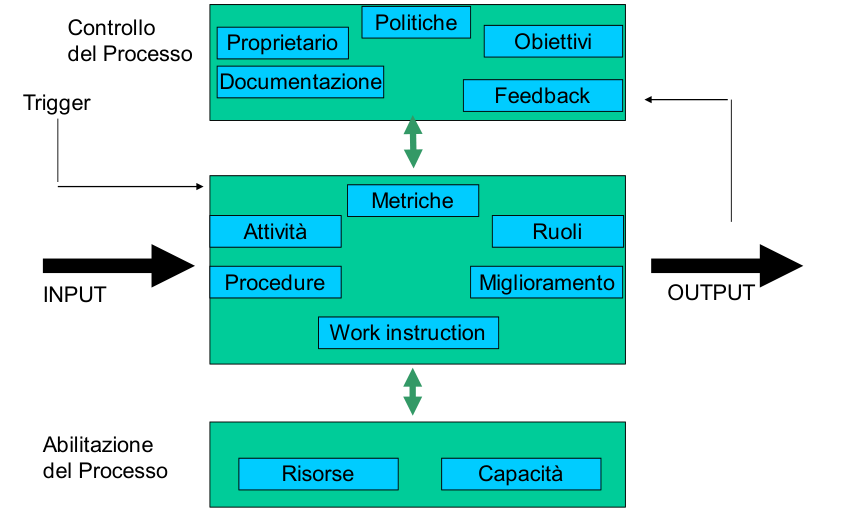
\includegraphics[scale=0.3]{images/caratteristiche_fondamentali_processo.png}
\end{figure}
Il processo è un'insieme di attività coordinate rivolte ad uno scopo specifico, per
produrre un risultato per creare valore direttamente o indirettamente per il cliente.


Per conoscere un processo bisogna conoscere \textbf{input}, \textbf{output}, \textbf{punti di monitoraggio}.

La struttura di un processo mostra:
\begin{itemize}
  \item Cosa deve essere fatto
  \item Risultati attesi
  \item Come misurare i risultati
  \item Come i risultati influenzano altri processi
\end{itemize}

Le caratteristiche fondamentali di un processo sono accumunabili in:
\begin{itemize}
  \item Essere \textbf{misurabile}
  \item Avere \textbf{risultati specifici}
  \item Avere \textbf{clienti}
  \item Rispondere a \textbf{eventi specifici}
\end{itemize}


\subsection{Controllo di un processo}
Il controllo di un processo è la sua pianificazzione per migliorarne l'efficienza,
inoltre ad ogni processo va assegnato un process owner.


\subsection{Efficienza ef efficacia di un processo}


\begin{align}
  \text{Efficienza} = \frac{\text{Output effettivo}}{\text{Input}}
\end{align}

\begin{align}
  \text{Efficacia} = \frac{\text{Output Effettivo}}{\text{Output atteso}}
\end{align}

\section{Flusso informatico e flusso informativo}

Il flusso informatico è di un processo è il flusso di informazioni associate ad un processo che passa diverse fasi.

Se il flusso informativo è completamente realizzato attraverso strumenti informatici si parla di \textbf{flusso informatico}.
